\documentclass[a4paper,11pt,handout]{beamer}

%%%%%%%%%%%%%%%%%%%%%%%%%%%%%%%%%%%%%%%%%%%%%%%%%%%%%%%%
% Change to 0 to produce only slides without the notes,%
% to 1 to generate an A4 document with the notes.      %
%%%%%%%%%%%%%%%%%%%%%%%%%%%%%%%%%%%%%%%%%%%%%%%%%%%%%%%%
\def\includeNotes{1}
%%%%%%%%%%%%%%%%%%%%%%%%%%%%%%%%%%%%%%%%%%%%%%%%%%%%%%%%

\usetheme{Pittsburgh}
\usecolortheme{whale}
\usepackage{siunitx}
\usepackage{graphicx}
\usefonttheme[onlymath]{serif}

\setlength{\parskip}{1em}

\graphicspath{{fig/}}

\setbeameroption{hide notes}
\setbeamertemplate{note page}[plain]
\usepackage{pgfpages}

% Define a layout to include 2 slides per page
\makeatletter
\define@key{pgfpagesuselayoutoption}{horizontal shift}%
{\def\pgfpageoptionhshift{#1}}
\define@key{pgfpagesuselayoutoption}{vertical shift}%
{\def\pgfpageoptionvshift{#1}}
\makeatother
\pgfpagesdeclarelayout{2 on 1 shifted}
{
	\edef\pgfpageoptionheight{\the\paperwidth} % landscaped by default
	\edef\pgfpageoptionwidth{\the\paperheight}
	\def\pgfpageoptionborder{0pt}
	\def\pgfpageoptionfirstshipout{1}
	\def\pgfpageoptionhshift{0pt}
	\def\pgfpageoptionvshift{0pt}
}
{
	\pgfpagesphysicalpageoptions
	{%
		logical pages=2,%
		physical height=\pgfpageoptionheight,%
		physical width=\pgfpageoptionwidth,%
		current logical shipout=\pgfpageoptionfirstshipout%
	}
	% stack on top of one another
	\pgfpageslogicalpageoptions{1}
	{%
		border shrink=\pgfpageoptionborder,%
		border code=\pgfusepath{stroke},%
		resized width=\pgfphysicalwidth,%
		resized height=.5\pgfphysicalheight,%
		center=\pgfpoint{.5\pgfphysicalwidth+\pgfpageoptionhshift}%
		{.75\pgfphysicalheight+\pgfpageoptionvshift}%
	}%
	\pgfpageslogicalpageoptions{2}
	{%
		border shrink=\pgfpageoptionborder,%
		resized width=\pgfphysicalwidth,%
		resized height=.5\pgfphysicalheight,%
		center=\pgfpoint{.5\pgfphysicalwidth+\pgfpageoptionhshift}%
		{.25\pgfphysicalheight+\pgfpageoptionvshift}%
	}%
}

\usepackage{ifthen}
\ifthenelse{\equal{\includeNotes}{1}}{%
	\pgfpagesuselayout{2 on 1 shifted}[%
		a4paper,border shrink=10mm, horizontal shift=0cm]
	\setbeameroption{show notes}}{}%


%%%%%%%%%%%%%%%%%%%%%%%%%%%%%%%%%%%%%%%%%%%%%%%%%%%%%%%%%%%

\title{Green communications in 5G}
\author{Tim Van Den Driesschen\\Rodrigo Arias Mallo}
\institute{Universitat Politècnica de Catalunya}
\date{\today}

\begin{document}

\begin{frame}
	\titlepage
\end{frame}
\note{}
%%%%%%%%%%%%%%%%%%%%%%%%%%%%%%%%%%%%%%%%%%%%%%%%%%%%%%%%%%%
\begin{frame}
\frametitle{Outline}

\begin{itemize}
	\item Introduction
	\item Main challenges
\item Network deployment
	\begin{itemize}
		\item Challenges 
		\item Potential solutions
	\end{itemize}
\item Renewable energy sources 
	\item Energy efficiency metrics
	\item Conclusions
\end{itemize}
\end{frame}
\note{%
}
%%%%%%%%%%%%%%%%%%%%%%%%%%%%%%%%%%%%%%%%%%%%%%%%%%%%%%%%%%%
\begin{frame}
\frametitle{Introduction}
\begin{itemize}

\item Meet the future requirements in an \textbf{affordable} and \textbf{sustainable} way
\item In the next decade, the number of connected devices is expected to 
increase 100 times and the  total data volume by \textbf{1000 times}

\item Operators are already facing \textbf{significant power bills}

\item Moving towards green communications is important both for 
\textbf{environmental} and \textbf{economic} reasons by \textbf{reducing CO2 emmisions  } and \textbf{saving money} 

\end{itemize}
\end{frame}
\note{
One of the big challenges is to meet future requirements and expectations in an affordable and sustainable way. Low energy consumption is the key to achieve this. Already today, the mobile operator’s energy bill is an increasing part of their OPEX (operational expenditure)

This is also important from a sustainability perspective; even though mobile communications today only contribute to a fraction of a percent of the global CO2 footprint [5], it is important to maintain or even reduce this in the future 5GrEEn [6] is a joint effort of partners tightly connected to the METIS project representing the telecom vendor Perspective.

This paper takes as a starting point the situation of today and tries to pinpoint important focus areas when designing an energy efficient 5G mobile network architecture. The outline is as follows: After a more in-depth discussion on major challenges for mobile networks in the future, the important focus areas and some potential solutions are outlined. Finally, a summary and concluding remarks are provided.
}
%%%%%%%%%%%%%%%%%%%%%%%%%%%%%%%%%%%%%%%%%%%%%%%%%%%%%%%%%%%
\begin{frame}
	\frametitle{Network planning and deployment}
    \begin{itemize}
\item Challenges
\begin{itemize}
\item Data traffic volumes
\item Number of connected devices
\item Diverse requirements of 5G
\item Energy consumption
\end{itemize}
\item Potential solutions
\begin{itemize}
\item Architectural design
\item Network deployment
\item Radio transmission
\item Backhauling solutions
\end{itemize}
\end{itemize}
\end{frame}
\note{%
Intro:

One of the big challenges is to meet future requirements and expectations in an affordable and sustainable way. Low energy consumption is the key to achieve this. Already today, the mobile operator’s energy bill is an increasing part of their OPEX (operational expenditure)

This is also important from a sustainability perspective; even though mobile communications today only contribute to a fraction of a percent of the global CO2 footprint [5], it is important to maintain or even reduce this in the future 5GrEEn [6] is a joint effort of partners tightly connected to the METIS project representing the telecom vendor Perspective.

This paper takes as a starting point the situation of today and tries to pinpoint important focus areas when designing an energy efficient 5G mobile network architecture. The outline is as follows: After a more in-depth discussion on major challenges for mobile networks in the future, the important focus areas and some potential solutions are outlined. Finally, a summary and concluding remarks are provided.

}
%%%%%%%%%%%%%%%%%%%%%%%%%%%%%%%%%%%%%%%%%%%%%%%%%%%%%%%%%%%

\begin{frame}
	\frametitle{Challenges: Data traffic Volumes}
    \begin{itemize}
\item Today: 2 billion mobile broadband subscriptions 
\item Exponential growth in the following years 
\item A factor of 1000x capacity demand in 2020 vs 2012  \begin{itemize}
\item Growing amount of users (10 times)
\item Growing amount of data rates per user (50 - 100 times)
\end{itemize}
\item Growing energy needs
\end{itemize}
\begin{center}
	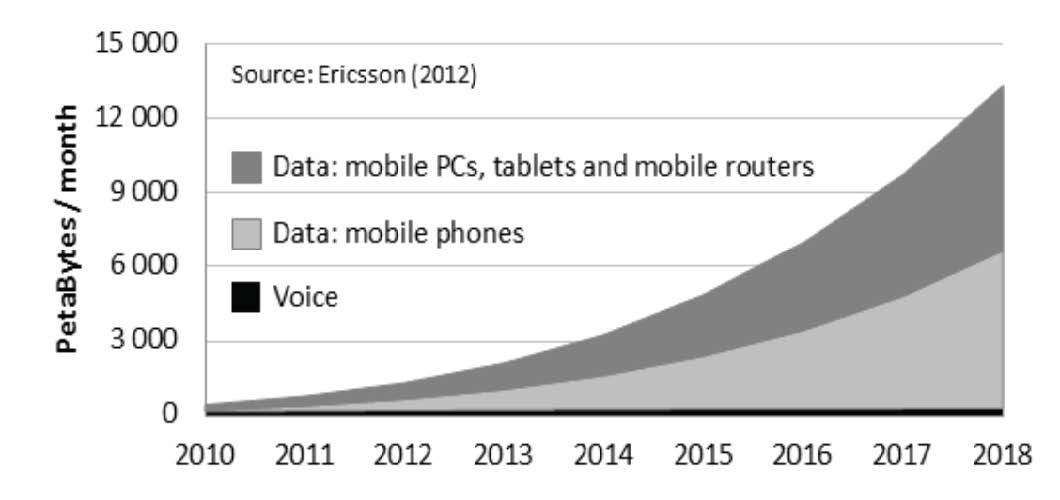
\includegraphics[scale=1]{Evolution_of_mobile_data_traffic_per_month_up_to_2018}
	\end{center}
\end{frame}

\note{Data traffic volumes:
Some of the challenges with regards to energy consumption is the growing amount of data traffic.
Today, there are over 2 billion mobile broadband subscriptions worldwide, a figure that has grown by 40 percent annually over the last six years.
Furthermore, forecasts predict that data traffic volumes will experience an exponential growth in the coming years [2], as illustrated in Fig. 1. For example, it can be seen that the data traffic volumes are expected to increase more than 10 times between 2012 and 2018. Predictions are made that per-user data rates are expected to grow by a factor of up to 50-100; on the other hand, the density of mobile Internet users is expected to increase by a factor of up to 10, implying a factor of 1000x capacity demand in the 2020 time frame
Hence, it is obvious that mobile systems in the future need to be capable of delivering significantly more capacity than today. 
In fact, up to now mobile networks were dimensioned by taking into account the peak
capacity. With this approach, the exponential growth rate will imply a costly network deployment. Instead, evolved mobile networks should satisfy the increasing traffic demand by a flexible availability of capacity (in time and space) in order to sustain the data rate development that has been observed during recent decades}
%%%%%%%%%%%%%%%%%%%%%%%%%%%%%%%%%%%%%%%%%%%%%%%%%%%%%%%%%%%

\begin{frame}
	\frametitle{Challenges: The number of connected devices}
        \begin{itemize}
\item Today:  7 billion mobile devices that are connected to the internet \begin{itemize}
\item Future: All connected through 5G connections
\end{itemize}  
\item  Smart devices (smart grid, sensors and surveillance camera's) 
\item Internet of things (IoT)
\end{itemize}
\begin{center}
	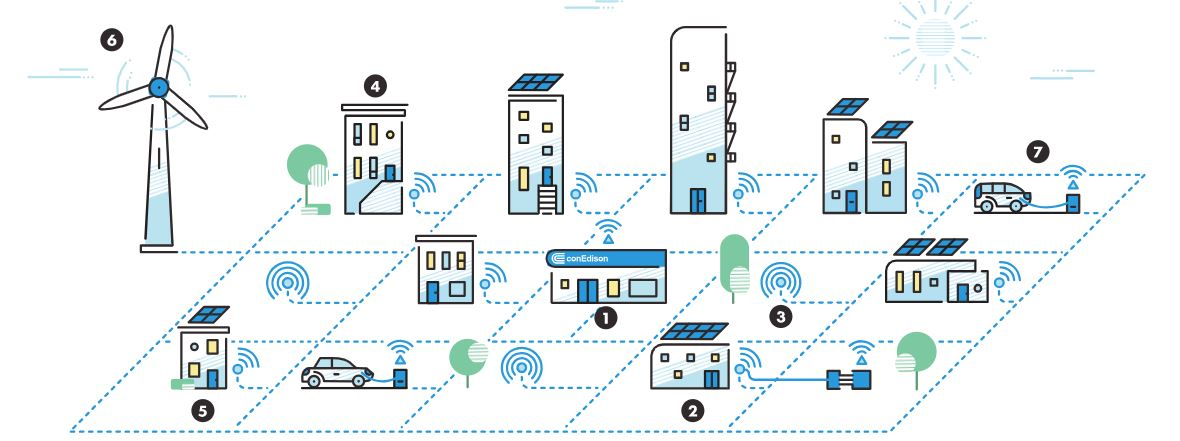
\includegraphics[scale=0.3]{Smart_grid}
\end{center}

\end{frame}
\note{
Today, there are almost 7 billion mobile subscriptions, and thereby wireless connected devices, worldwide.

However, in the future, this is predicted to change, as different kinds of machines such as smart grid devices, sensors and surveillance cameras will be connected to the networks. 

This is usually referred to as Internet-of-things [3] or machine-to-machine (M2M)
communication, and means that everything that can benefit from a wireless connection will have a wireless connection
}
%%%%%%%%%%%%%%%%%%%%%%%%%%%%%%%%%%%%%%%%%%%%%%%%%%%%%%%%%%%
\begin{frame}
	\frametitle{Challenges: Diverse requirements}
            \begin{itemize}
\item Different applications of 5G
\begin{itemize}
\item Low latency 
\item High reliability
\item Different data sizes (e.g. security cameras (large) and temperature sensor (small))
\item Varying quality of service (QoS) requirements
\begin{itemize}
\item Green energy should not have a negative impact on the QoS
\end{itemize}
\end{itemize}
\end{itemize}
\begin{center}
	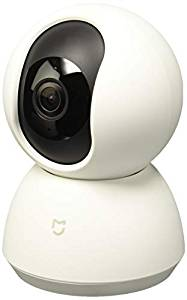
\includegraphics[scale=0.4]{Smart_camara} 
    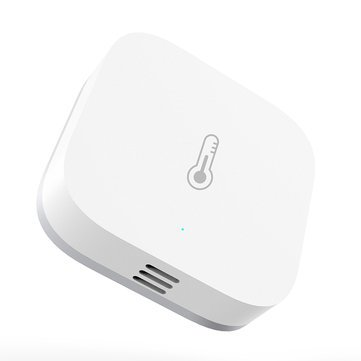
\includegraphics[scale=0.3]{Smart_temp}
\end{center}
\end{frame}
\note{
Challenges:
5G will include a myriad of applications with a wide range of requirements and characteristics.

Some applications may require low latency, for example, time-critical control functions in industrial applications. The same type of applications typically also require very high reliability, while others such as simple sensors can have lower reliability requirements. Certain applications such as surveillance cameras may have to convey enormous amounts of data while others have very small data amount to send.

varying quality-of-service (QoS) requirements. This may have a significant impact on
the green design, as the minimization of network power consumption, should not have impacts on the correct and efficient management of the QoS in the system.


}
%%%%%%%%%%%%%%%%%%%%%%%%%%%%%%%%%%%%%%%%%%%%%%%%%%%%%%%%%%%
\begin{frame}
	\frametitle{Challenges: Energy consumption}
    \begin{itemize}
    \item Operational expenditure (OPEX)
    \item The energy consumption should at least be kept at the same level as today
    	\begin{itemize}
    	\item Increasing number of devices
    	\item Increasing number of traffic 
   		\item New requirements 
\end{itemize}

\end{itemize}
\end{frame}
\note{
Challenges: Energy consumption:
Already today, the mobile operator’s energy bill is a substantial and increasing part of their OPEX,
The energy consumption should at least be kept at the same level as today (despite the traffic growth, the massive amount of devices, and new requirements)
The EARTH project showed that it is possible to cut the energy consumption of
LTE by a factor of 4 with a 2012 baseline [10].

5GrEEn will target a factor of 10 lower energy consumption compared to today while fulfilling the requirements stated in the previous subsections.


}
%%%%%%%%%%%%%%%%%%%%%%%%%%%%%%%%%%%%%%%%%%%%%%%%%%%%%%%%%%%
\begin{frame}
	\frametitle{Potential solutions: Architectural design }
    \begin{itemize} 
\item Architectural design
\begin{itemize}
\item An energy efficient system needs to be efficient both when transmitting data as well as when we are not transmitting data
\item logical separation between idle mode functions and user plane data transmission
\end{itemize}

\item Dynamic cells with reconfigurable antenna systems 
\end{itemize}
\begin{center}
	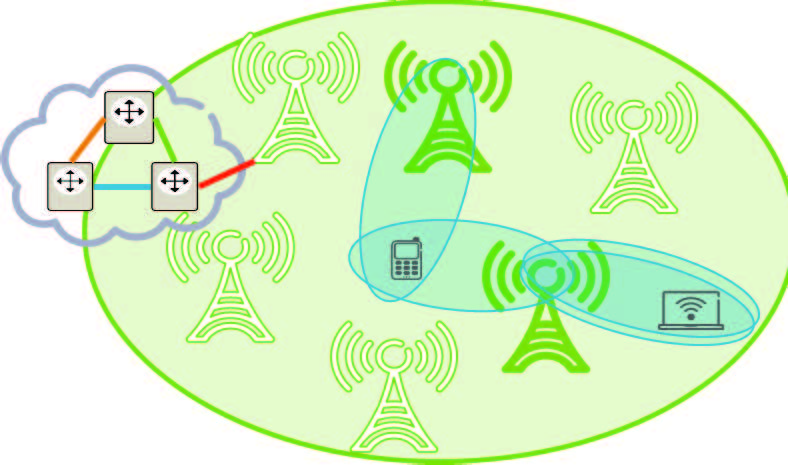
\includegraphics[scale=1]{Logical_separation_between_idle_mode_and_active_mode_network}
	\end{center}    
    
\end{frame}
\note{
Challenges:
Equations:
An energy efficient system needs to be efficient both when transmitting data as well as when we are not transmitting data. 

To do this, we will assume a logical separation between idle mode functions (such as the transmission of system information) and user plane data transmission and reception, see Fig. 2.
In this architectural design, cells can be viewed as UE specific resources for data transfer that are dynamically created and configured to support only the currently active UEs. 

Moreover, an access point may be utilized by more than one cell. Also, a dynamic cell may fully utilize a reconfigurable antenna system (using e.g. beam-width and tilt optimization) at the access point(s) in order to shape the coverage in the best way.

The control plane carries control information (also known as signalling); the user plane carries the network's users’ traffic; the management plane carries the operations and administration traffic required for network management. Broadcast of
system information also belongs to the management plane. By separation of the network into these planes we facilitate e.g. independent utilization of access points by the planes, i.e. a given access point may be used by a subset of the planes. 
Hence independent deployment of the different plane entities can be done at the
most energy efficient location.


}
%%%%%%%%%%%%%%%%%%%%%%%%%%%%%%%%%%%%%%%%%%%%%%%%%%%%%%%%%%%
\begin{frame}
	\frametitle{Potential solutions: Network Deployment}
    \begin{itemize}
    \item Heterogeneous network deployment \begin{itemize}
\item Small cells are deployed under an umbrella of macro cells
\item Small cells offload macro cells --> overall energy saving 
\item Improves coverage in areas 
\end{itemize}
\item Deployment is interesting in places where high data rates are needed (e.g. Shopping malls and train stations)\begin{itemize}
\item Indoor places
\item Energy savings due to avoidance of power consuming wall penetration
\end{itemize}
    \end{itemize}
    
\end{frame}
\note{
Challenges:
Energy efficiency improvements through network deployment strategies have been touched upon in several projects for state-of-art technologies.

Especially heterogeneous network deployments, where small cells are deployed under an umbrella macro-cellular coverage, have gained great interest and have been presented as a promising solution for improving energy efficiency of LTE [13]. This is due to the fact that if correctly placed the small cells can significantly offload the macro cells with an overall energy saving as result. In order to handle the future capacity demands and the massive amounts of different devices, it is expected that even denser deployments, so-called ultra-dense deployments (see Fig. 3), will be necessary. 
These deployments are of particular interest in areas where extremely high data rates and capacity are needed, for example in offices, shopping malls, and subway stations. As these typically are located indoor, we can expect this to be beneficial from an energy consumption perspective due to the avoidance of power consuming wall penetration.

If care is not taken in the design a small cell deployment can still result in increased energy consumption.

5GrEEn will develop energy-optimized heterogeneous network deployment strategies for different traffic distributions and environments that will provide capacity where it is actually needed and will bring maximum benefit from the additional flexibility created by the new system architecture.

Future network dimensioning will not only consider the busy hour traffic and aim to minimize the total power consumption for the worst case scenario -as is currently being applied- but it will take the daily traffic variation into account to minimize the overall energy consumption. New network deployment solutions need to be developed that minimize the energy consumption through long- and short-term sleep opportunities by exploiting the flexibility in the new system architecture. 

}
%%%%%%%%%%%%%%%%%%%%%%%%%%%%%%%%%%%%%%%%%%%%%%%%%%%%%%%%%%%
\begin{frame}
	\frametitle{Potential solutions: Radio Transmissions}
    \begin{itemize}
    \item Avoid sending signals in directions with no receivers
\item Multiple-input multiple-output (MIMO) transmission
\item Beam forming 
\item MIMO --> Will boost peak data rates \begin{itemize}
\item Boost peak data rates
\item Higher data rates mean more time to sleep
\item Higher data rates mean less base stations are necessary 
\end{itemize}
    \end{itemize}
\end{frame}
\note{
As already mentioned in the system architecture section above, an energy efficient system needs to be efficient both when transmitting data as well as when we are not
transmitting data. In order to be energy efficient when transmitting data, all we need to do is to “send the packet to the receiver”. We should do it quickly and we should try to avoid sending signals in directions that do not reach the receiver.

Multiple-input multiple-output (MIMO) transmission which allows both multi-layer transmission for increased data rates, and beamforming to a certain extent.
We believe that the MIMO technology has further potential. Recently, massive antenna configurations, or very large MIMO, have gained increased interest.

MIMO will further boost peak data rates and system capacity, which can benefit energy efficiency in two ways; higher peak data rates mean more time for sleep, higher system capacity means that a future traffic demand can be served without a corresponding densification of the network.

Such high gain beamforming, in combination with the system architecture solutions mentioned above, can allow increased inter-site distances with maintained system capacity, which of course is beneficial from an energy efficiency point of view.

}
%%%%%%%%%%%%%%%%%%%%%%%%%%%%%%%%%%%%%%%%%%%%%%%%%%%%%%%%%%%
\begin{frame}
	\frametitle{Potential solution: Bachhauling }
    \begin{itemize}
    \item Trade-off between power saved by using small and low power base stations and the baseline power that has to be spent to backhaul their traffic
    \end{itemize}
    \begin{center}
	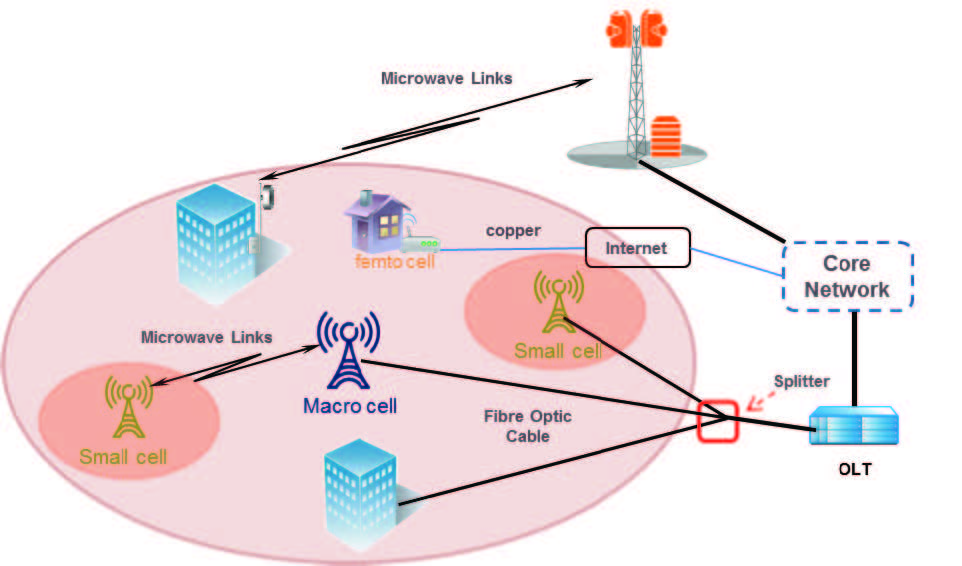
\includegraphics[scale=1]{Illustration_of_possible_backhauling_solution}
	\end{center} 
\end{frame}
\note{
Backhauling Solutions 
Despite the relative scarce attention paid to the role of backhaul in optimizing the overall power budget of mobile radio networks, recent studies have highlighted its remarkable impact especially when heterogeneous deployments are considered [18]. The results showed that there is a trade off between the power saved by using small and low power base stations and the baseline power that has to be spent to backhaul their traffic.

In 5GrEEn, we will tackle these questions and study various existing and future backhaul technologies. We will consider the advantages/disadvantages of different backhaul technologies, e.g., microwave, fibre, copper, for different deployment scenarios as shown in Fig. 4.
For example, fibre-based backhaul has higher CAPEX and longer deployment
time but offer long-term support with respect to increasing capacity requirements. Microwave is an appealing solution due to its quick and relatively cheap deployment potential. On the other hand, there is still a great interest in copper based solution in order to increase their capacity so that the existing infrastructure can still be exploited at its maximum. Therefore, a “one solution fits all” may not be viable.

The result of a mix of fiber, microwave and copper, depending on several factors, e.g., existing infrastructure, spectrum and license costs, availability of equipment, operator business modeling, and QoS level to be provided.

With this knowledge, it will also be possible to define new and holistic wireless deployment strategies tailored for specific back haul architectures to avoid the bottleneck in the back haul power consumption.

}
%%%%%%%%%%%%%%%%%%%%%%%%%%%%%%%%%%%%%%%%%%%%%%%%%%%%%%%%%%%
\begin{frame}
\frametitle{Reducing power consumption [181]}
	\begin{center}
	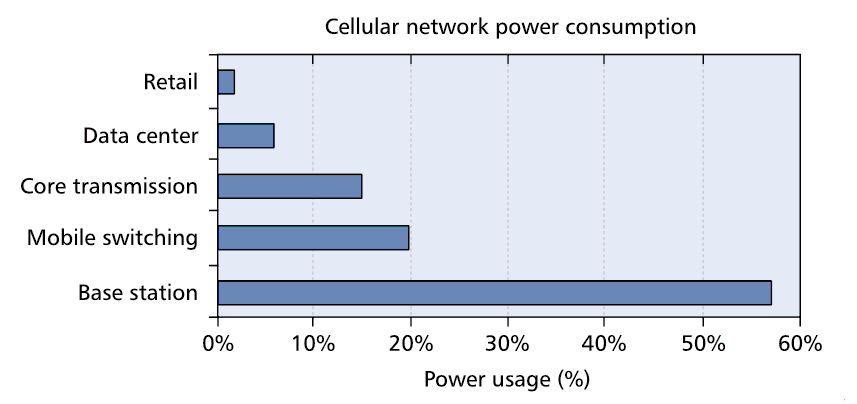
\includegraphics[scale=1]{consumption.png}
	\end{center}

\begin{itemize}

	\item The base station is the most power intensive element (more than 50\%).
	\item Also the usual lifetime is around 10--15 years, while smartphones is only 2.
	\item By reducing the power consumption of the largest element, the whole 
	consumption is reduced.

\end{itemize}
\end{frame}
\note{

}
%%%%%%%%%%%%%%%%%%%%%%%%%%%%%%%%%%%%%%%%%%%%%%%%%%%%%%%%%%%
\begin{frame}
\frametitle{Harvesting renewable energy resources}
In order to power the Base Stations (BS), energy can be obtained from renewable 
sources:

\begin{itemize}
\item Natural sources: Sun, wind, vibration
\item External: Batteries, fuel cells
\end{itemize}
\end{frame}
\note{%
Solar energy has been studied in UK cities, in order to power BS installed in 
road lamps, with a solar panel on top [175]. It has been observed that it can 
run fully autonomous, with the exception of the January month, where external 
power was needed.

Other sources of energy may not be so profitable, as sun is the source with the
highest amount of power, about \SI{100}{\milli\watt\per\centi\meter\squared}, 
followed by the wind with \SI{12}{\milli\watt\per\centi\meter\squared}.
}
%%%%%%%%%%%%%%%%%%%%%%%%%%%%%%%%%%%%%%%%%%%%%%%%%%%%%%%%%%%
\begin{frame}
\frametitle{Power density}
	\begin{center}
	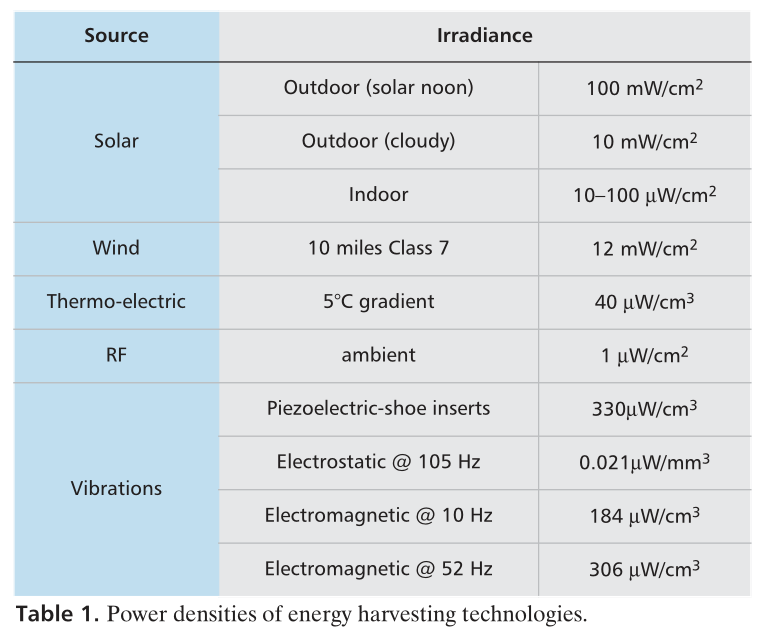
\includegraphics[width=.8\textwidth]{power-density.png}
	\end{center}

\end{frame}
\note{%
Other sources of energy are shown in the table, but we observe the best ones are 
the solar and wind, with orders of magnitude far from the rest. }
%%%%%%%%%%%%%%%%%%%%%%%%%%%%%%%%%%%%%%%%%%%%%%%%%%%%%%%%%%%
\begin{frame}
	\frametitle{Smaller frame overhead %
		\footnote{Following [178] paper in depth: Uplink Contention Based Multiple 
		Access for 5G Cellular IoT}%
	}

	\begin{itemize}
		\item Bursty traffic cause devices to change state between idle and 
		connected with the associate \textbf{power consumption}
		\item Significant \textbf{overhead} with small packets
		\item Contention based method have been proposed
		\end{itemize}
\end{frame}
\note{Expand based on reference 178}
%%%%%%%%%%%%%%%%%%%%%%%%%%%%%%%%%%%%%%%%%%%%%%%%%%%%%%%%%%%
\begin{frame}
	\frametitle{Uplink contention based methods}


	\begin{center}
	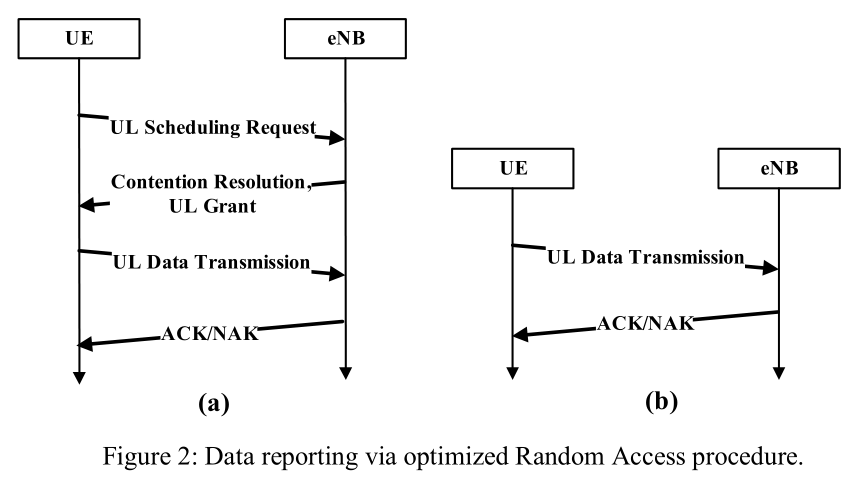
\includegraphics[scale=0.3]{uc.png}
	\end{center}

	\begin{itemize}
		\item Small signalling payload
		\item Direct small data packet
	\end{itemize}
\end{frame}
\note{}
%%%%%%%%%%%%%%%%%%%%%%%%%%%%%%%%%%%%%%%%%%%%%%%%%%%%%%%%%%%
\begin{frame}
	\frametitle{Results of simulation}

	\begin{center}
	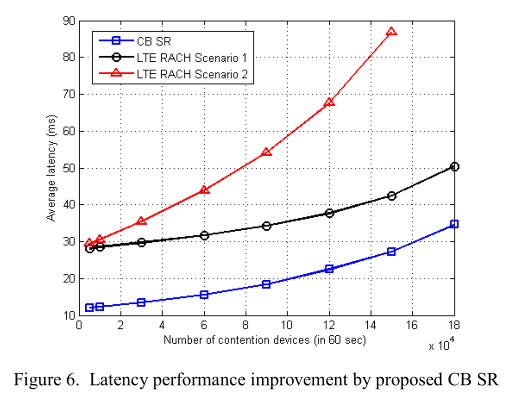
\includegraphics[scale=0.4]{cb-latency.png}
	\end{center}

\end{frame}
\note{}
%%%%%%%%%%%%%%%%%%%%%%%%%%%%%%%%%%%%%%%%%%%%%%%%%%%%%%%%%%%
\begin{frame}
\frametitle{Open problems}

\begin{itemize}
\item Power control: max power BS, sunlight.
\item Energy efficient hardware: transceivers
\item Energy efficient network architecture: SDN, NFV, data/control plane
\item New battery technologies: sugar bio-batteries%
\footnote{Following [183] paper in depth: \textsl{A high-energy-density sugar 
biobattery based on a synthetic enzymatic pathway}}, photo-MFC
\end{itemize}

\end{frame}
\note{
There are some challenges to be resolved.
\begin{itemize}
	\item Power control
	\begin{itemize}
		\item In multi-tiered networks, the user is not connected to the BS with 
		maximum power.
		\item Solar and wind energy harvesting can be unfeasible in dense localities 
		and where sunlight is not available.
	\end{itemize}
	\item Energy efficient hardware
	\begin{itemize}
		\item Current transceivers are energy costly, as they are designed for good 
		throughput.
	\end{itemize}
	\item Energy efficient network architecture
	\begin{itemize}
		\item Multiple technologies as MIMO, SDN, NFV, D2D, cloud computing...
		\item Separation of control and data planes
		\end{itemize}
	\item New battery technologies: sugar bio-batteries, photo-MFC%
	\begin{itemize}
		\item Based on enzymes that extract energy from sugar, similar to humans.
		\item Moss can also be used to harvest solar power
		\item Still with a low efficiency to be used.
	\end{itemize}
\end{itemize}
}
%%%%%%%%%%%%%%%%%%%%%%%%%%%%%%%%%%%%%%%%%%%%%%%%%%%%%%%%%%%
\begin{frame}
\frametitle{Sugar bio-batteries [183]}

	\begin{center}
	
\includegraphics[scale=0.3]{trash.jpg}
	\end{center}

\begin{itemize}

	\item The typical density of energy of a Lithium cell is around 
	\SI{0.54}{\mega\joule\per\kilogram}

	\item But the combustion energy of glucose can release up to 
	\SI{15.5}{\mega\joule\per\kilogram}

	\item Sugars are non toxic, safe and carbon neutral

\end{itemize}
\end{frame}
\note{
The energy per Kilogram stored in a lithium cell is about 2 orders of magnitude 
below the available energy in an equivalent sized glucose cell.

Experiments with bio-batteries seem to have a suitable position as power cells, 
however the research is in an early stage of development.
}
%%%%%%%%%%%%%%%%%%%%%%%%%%%%%%%%%%%%%%%%%%%%%%%%%%%%%%%%%%%
\begin{frame}
\frametitle{Sugar bio-batteries [183]}

\begin{itemize}

	\item Maltodextrin (food additive), produced from starch.
	\item Sugars are non toxic, safe and carbon neutral
	\item The lifetime of enzymes is very short (weeks)
	\item They have to be recharged regularly.

\end{itemize}
\end{frame}
\note{
The main idea of the cells, is as follows. The sugar is used as fuel, some 
enzimes ar used to transform the glucose into othe compounds, while energy is 
released in form of electric current.

Those cells are able to work for long periods with a suitable flow of 
glucose-like input stream. The enzymes used for the transformation of sugar are 
non toxic, an easy to obtain, they don't need any exotic metal nor element.
}

%%%%%%%%%%%%%%%%%%%%%%%%%%%%%%%%%%%%%%%%%%%%%%%%%%%%%%%%%%%
\begin{frame}
\frametitle{Sugar bio-batteries [183]}

	\begin{center}
	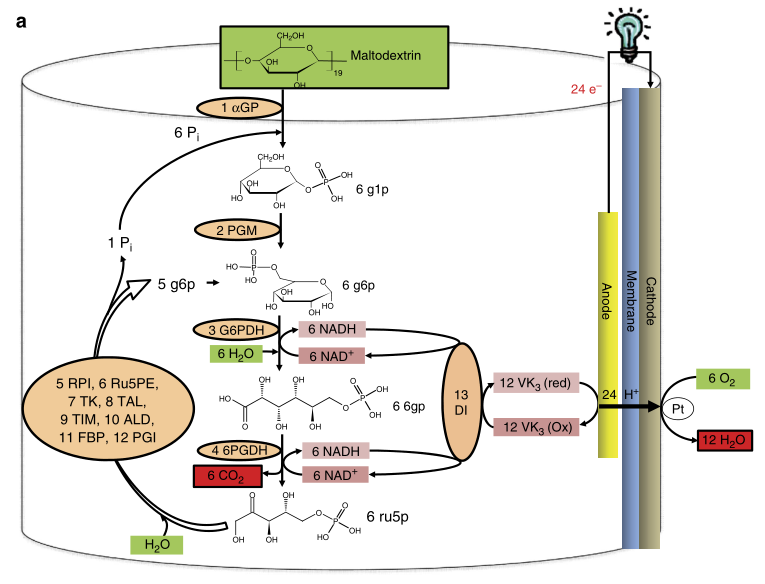
\includegraphics[width=.9\textwidth]{cicle.png}
	\end{center}

\end{frame}
\note{
With a suitable input stream of sugars, those cells can keep producing a long 
term power output. The two electrodes placed close to the chemical reaction 
obtain the electric energy directly from the enzimes.
}
%%%%%%%%%%%%%%%%%%%%%%%%%%%%%%%%%%%%%%%%%%%%%%%%%%%%%%%%%%%



\begin{frame}
\frametitle{Energy efficiency metrics [179]}

\begin{itemize}

	\item We need some way to compare energy efficiency (EE), but which metric is 
more suitable?
	\item Output energy/input energy?
	\item Performance/energy consumption?
	\item What load should we use for the measurement?
	\item Accuracy?

\end{itemize}
\end{frame}
\note{
In order to obtain an meaningful comparison of different technologies used in 
electronic communications, some metrics should be established so we can compare 
the energy efficiency.

Some candidates as the output power by the input power are useful when we can 
measure the power, but some times other measurements are more interesting. For 
example if we look at a processing unit, we may be interested in the performance 
per watt.

The base stations can operate at different loads, and the metric should include 
information of the load to be compared. Also the accuracy of the metric should 
be taken into consideration, as it may include information of fluctuations when 
the system is under operation.

We will focus on the metrics used at different levels of abstraction, starting 
from the lowest part, the component level, to the uppermost, the network level.
}
%%%%%%%%%%%%%%%%%%%%%%%%%%%%%%%%%%%%%%%%%%%%%%%%%%%%%%%%%%%
\begin{frame}
\frametitle{EE at component level}

	\begin{figure}[h]
	\begin{center}
	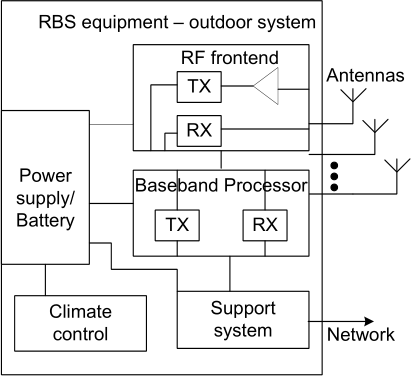
\includegraphics[scale=0.3]{ee-component.png}
	\end{center}
	\end{figure}

\begin{itemize}

	\item The components are analyzed by parts
	\item Example: The efficiency of the antenna as the input power that it 
receives compared with the irradiated power.
	\item On the baseband processor, EE is measured as performance per unit of 
energy consumption.
	\item For the power supply, output power/input power, often higher than 
85\%

\end{itemize}
\end{frame}
\note{
A general model is commonly used, as the one in the figure, to understand the 
different parts of a system. In each part we can identify and measure the 
efficiency based on specific metrics.

In the case of a radio base station, which may include one or more antennas, the 
efficiency can be expressed as the ratio of the radiated power $P_r$ to the 
input power $P_i$, $$ \eta = P_r / P_i$$

Whereas, in a baseband processor we are interested in the performance per watt, 
which can be measured by means of MFLOPS or MIPS which often can be expressed in 
equivalent MOPS (millions of operations per second).

The power supply is normally measured in terms of electrical efficiency, with 
the ration of output power by input power, often higher than 85\%.
}
%%%%%%%%%%%%%%%%%%%%%%%%%%%%%%%%%%%%%%%%%%%%%%%%%%%%%%%%%%%
\begin{frame}
\frametitle{EE at equipment level}

\begin{itemize}

	\item Power is computed by each load level (high, med, low).
	\item Power supply correction factor and cooling factor.
	\item Energy consumption rating: Power/effective throughput.

\end{itemize}
\end{frame}
\note{
The power consumption can be sampled at different load conditions, for example 
high or busy hour, medium and low usage. Then the power consumption is averaged 
with the time of each load estimation, giving a more realistic power 
consumption.

Both the power supply and cooling factor are unit specific and can be used to 
correct the estimated power usage.

The European Telecommunications Standards Institute (ETSI) doesn't provide an 
energy efficiency metric for radio base stations, but the Energy Concumption 
Rating (ECR) iniciative proposes the power consumption $P$ by throughput $T$ in 
bits per seconds, $ECR = P/T$
}
%%%%%%%%%%%%%%%%%%%%%%%%%%%%%%%%%%%%%%%%%%%%%%%%%%%%%%%%%%%
\begin{frame}
\frametitle{EE at network level}

\begin{itemize}

	\item Rural, cellular: Coverage area/average power consumption
	\item Urban: Subscribers/average power consumption
	\item Error correction: transmitter power/bit rate

\end{itemize}
\end{frame}
\note{
Wireless systems like cellular networks are deployed with careful network 
planning. Coverage area in rural areas should be considered, whereas in urban 
areas we often exceed the capacity of the systems.

For the rural and cellular networks, the following EE metric can be used: The 
area of coverage $A$ by the power consumption $P_c$, defined as $P = A/P_c$.

However for a urban network, we may be interested in the number of suscribers 
$N$ by the power consumption $P_c$, defined as $P = N / P_c$

On the other hand, the usage of error correcting codes can have an impact in the 
energy consumption. The EE metric $E = P/C$ is based on the transmitter power 
$P$ and the bit rate $C$ of the channel.}
%%%%%%%%%%%%%%%%%%%%%%%%%%%%%%%%%%%%%%%%%%%%%%%%%%%%%%%%%%%
\begin{frame}
\frametitle{Conclusions}

\begin{itemize}
	\item 5G communications are possible: open problems have potential solutions.
	\item New technologies and research is still needed.
	\item Energy efficiency can be improved by several methods.
	\item Standarized metrics lead to reasonable comparison of efficiency.
\end{itemize}
\end{frame}
\note{
While the development of 5G communications seem daunting at least, the presented 
open problems have multiple potential solutions. It is expected that more 
research is required to implement them, while we develop new technologies.

In order to reduce the energy usage, we have seen different energy harvesting 
methods as well as energy efficient systems, designed to keep our CO$_2$ 
footprint at minimum.

With the standarization of new metrics for energy efficiency, we expect more 
competitive hardware to be replaced in the coming years.
}
%%%%%%%%%%%%%%%%%%%%%%%%%%%%%%%%%%%%%%%%%%%%%%%%%%%%%%%%%%%

\end{document}

